\documentclass[11pt]{article}
\usepackage[margin=1in]{geometry}
\usepackage{amsmath,amssymb}
\usepackage{booktabs}
\usepackage{graphicx}
\usepackage{hyperref}
\usepackage[T1]{fontenc}
\newcommand{\code}[1]{\texttt{#1}}
\title{Pale Bands in the Affine Heatmaps:\\
What They Are, and the Search for Hidden Computation}
\author{local\_mixing working notes}
\date{2026-08-02}

\begin{document}
\maketitle

\begin{abstract}
Reading the layer-2 profile sweep's heatmaps at pixel resolution turned up
narrow vertical bands where the mixed circuit is markedly less
affine-readable. This note establishes what they are. Three results, in
order of importance. (1) The heatmap measure carries \emph{no sampling
noise}: every cell is an exact count of non-recoverable target bits, and
the plate is byte-identical under different random seeds --- so every
visible feature is real structure, and the ``is it jitter'' question is
answered before it is asked. (2) The bands are genuine local regions,
200--2200 gates wide, where 40--75 more of the 512 target bits go
unreadable. (3) They are \emph{dead}, not \emph{hidden}: a whole-circuit
search across every position and every gap width up to 11k gates finds no
case where the computation re-emerges further along, with the observed
statistic sitting far \emph{below} its own null. The interesting
phenomenon --- mixed material performing part of the source computation
invisibly --- does not occur in this mixer's output at any measurable
resolution.
\end{abstract}

\section{The instrument has no noise floor}

\code{hmap\_affine} scores cell $(i,j)$ by fitting, for each of the $n$
target bits of $C$'s prefix $i$, a GF(2) affine function of the mixed
circuit's wires at prefix $j$: inconsistent (the bit is not affine in those
wires) scores $0.5$; consistent scores the measured holdout error, which is
$\approx 0$ for a genuine affine relation. So
\[
H(i,j) \;=\; \tfrac{1}{2}\cdot\bigl(\text{fraction of $C$'s bits not
affine-recoverable from $G_j$}\bigr).
\]

Two checks confirm this is exact rather than statistical:

\begin{itemize}
\item \textbf{Quantisation.} Every cell of the $101 \times 121$ \code{nR30}
plate is an exact integer multiple of $0.5/n = 0.5/512 = 0.000977$
--- 100\% of cells on the lattice, to within $10^{-3}$ of a multiple.
\item \textbf{Seed independence.} Runs at seeds 12345, 999, 4242 and 31337
produce \textbf{byte-identical} \code{.bin} files, as does a minimal control
at seeds 7 and 88888. Span membership over GF(2) is a fact about the
functions, not about which random inputs were drawn.
\end{itemize}

Consequence: there is no noise to discount. A column that looks pale
\emph{is} pale. (An earlier ``how many standard errors'' framing in this
investigation was therefore mis-conceived, and is superseded.)

\emph{Caveat worth carrying:} because the plate is seed-independent, one
cannot use re-seeding to cross-check a feature, and agreement between the
degree-1 and degree-2 plates is \textbf{not} independent evidence --- both
draw their sample batches from the same seeded stream, so the degree-2
run's first 96 batches are byte-identical to the degree-1 run's.

\section{What the bands are}

\subsection{Width and depth}

On the coarse plate (column spacing 1876 gates) 17 of 121 columns sit more
than $2$ local units above baseline. Re-measured at 200-gate spacing
($26 \times 1127$), the features resolve into structured bands with smooth
shoulders:

\begin{table}[h]\centering\small
\begin{tabular}{lrrr}
\toprule
$G$-gate range & width (gates) & peak $H$ & peak non-recoverable bits \\
\midrule
13{,}200--15{,}200 & 2{,}200 & 0.3941 & \textbf{404} of 512 \\
97{,}600--98{,}800 & 1{,}400 & 0.3805 & 390 \\
178{,}200--178{,}800 & 800 & 0.3837 & 393 \\
20{,}800--21{,}400 & 800 & 0.3853 & 395 \\
125{,}200--125{,}600 & 600 & 0.3622 & 371 \\
four more & 200--400 & 0.367--0.372 & 377--381 \\
\midrule
typical material & --- & 0.3226 & 330 \\
\bottomrule
\end{tabular}
\caption{\code{nR30}. The ordinary column-to-column wobble on this plate is
7.5 bits of 512; the bands stand well clear of it.}
\end{table}

\subsection{They appear in every arm}

Each of the eight profile arms has them; \code{nR30} merely has the most,
and its larger circuit spaces them far enough apart to be seen separately.
Per-arm strongest band (excluding edge columns), all rendered at matched
aspect and a common colour scale:

\begin{center}\small
\begin{tabular}{lrrrr}
\toprule
arm & size ratio & band $G$ & peak $H$ & bits \\
\midrule
no twist & 1.30 & 40{,}145 & 0.3535 & 362 \\
R1=1.5 & 1.49 & 6{,}230 & 0.3611 & 370 \\
R1=2.0 & 1.79 & 137{,}700 & 0.3605 & 369 \\
R1=2.5 & 1.99 & 6{,}648 & 0.3808 & 390 \\
R1=3.0 & 2.25 & 97{,}552 & 0.3684 & 377 \\
short hold & 1.62 & 37{,}800 & 0.3501 & 359 \\
long hold & 1.98 & 108{,}636 & 0.3467 & 355 \\
10$\times$ twist & 6.42 & 176{,}484 & 0.3632 & 372 \\
\bottomrule
\end{tabular}
\end{center}

\subsection{Framing note: the plate's aspect is the size ratio}

The ridge's slope is $\mathrm{d}G/\mathrm{d}C = |G|/|C|$. For \code{nR30}
that is $225{,}014/100{,}000 = 2.25$, and the measured ridge slope is
$2.183$ (fractional slope $0.970$) --- the diagonal crosses corner to
corner, as it must. A local window therefore needs its $G$ extent to be
$\approx 2.25\times$ its $C$ extent or the ridge sweeps out of frame; the
first round of zoom plates in this investigation was mis-framed for exactly
this reason. The per-row ratio also drifts from $2.63$ early to $2.25$ late,
i.e.\ material that was present early is proportionally more inflated ---
a residue of the expansion phase that compression did not re-flatten.

\section{Dead, not hidden}

\subsection{The question}

A pale band where the ridge resumes at the \emph{same} $C$ position is
uninteresting: it is a stretch that does no work (an identity, in effect).
The interesting event would be a band after which the computation
\textbf{re-emerges further along} --- mixed material that performed part of
$C$ invisibly and handed back the result. That is a specific, testable
signature: a persistent forward level-shift in the ridge trajectory
$C^*(G)$, beyond what the size ratio predicts.

\subsection{The search}

Two whole-circuit plates at $501 \times 641$ cells ($C$ step 200 gates,
$G$ step 280--352), so the detector scans \emph{every} position rather than
a hand-picked window. For each candidate position the trend fitted on the
left of the gap is extrapolated across it and compared with the level on the
right; the gap width is swept from 1 to 32 columns (352 up to 11{,}264
gates). The null detrends the true ridge and \emph{shuffles its residuals},
preserving the wobble's magnitude while destroying its structure, then runs
the identical detector.

\begin{table}[h]\centering\small
\begin{tabular}{lrrrrr}
\toprule
circuit & gap (gates) & observed & null p95 & null max & $p$ \\
\midrule
\code{nR30} & 352 & 1{,}125 & 4{,}418 & 4{,}837 & 1.000 \\
\code{nR30} & 2{,}816 & 2{,}525 & 7{,}518 & 8{,}273 & 1.000 \\
\code{nR30} & 11{,}264 & 5{,}783 & 17{,}764 & 19{,}677 & 1.000 \\
\code{nR20} & 280 & 875 & 2{,}298 & 2{,}888 & 1.000 \\
\code{nR20} & 2{,}240 & 2{,}075 & 3{,}916 & 4{,}529 & 1.000 \\
\code{nR20} & 8{,}960 & 6{,}175 & 9{,}624 & 11{,}376 & 0.950 \\
\bottomrule
\end{tabular}
\caption{Largest persistent forward shift in $C$ gates. Every cell $p \ge
0.95$.}
\end{table}

\subsection{Verdict}

No re-emergence events, at any scale, anywhere in either circuit. The result
is stronger than a bare null: the observed statistic sits \emph{far below}
its own null distribution, typically a quarter to a half. Shuffling destroys
the autocorrelation of the ridge's wobble and manufactures apparent leaps
that the true trajectory never makes --- the real ridge is
\textbf{smoother than chance}. $C$'s computation advances steadily at the
size-ratio rate; the bands are stretches where it does not advance and then
resumes exactly where it left off.

An earlier pass of this analysis, restricted to eight 6000-gate windows,
appeared to find persistent shifts of 430--820 $C$-gates in all eight arms.
That was the maximum of a noisy statistic over $\sim$120 candidate
positions, and the null test dissolved it ($p = 0.05$ to $1.00$). It is
recorded here because the failure mode --- cherry-picking an extremum
without a null --- is the one this kind of search invites.

\begin{figure}[h]\centering
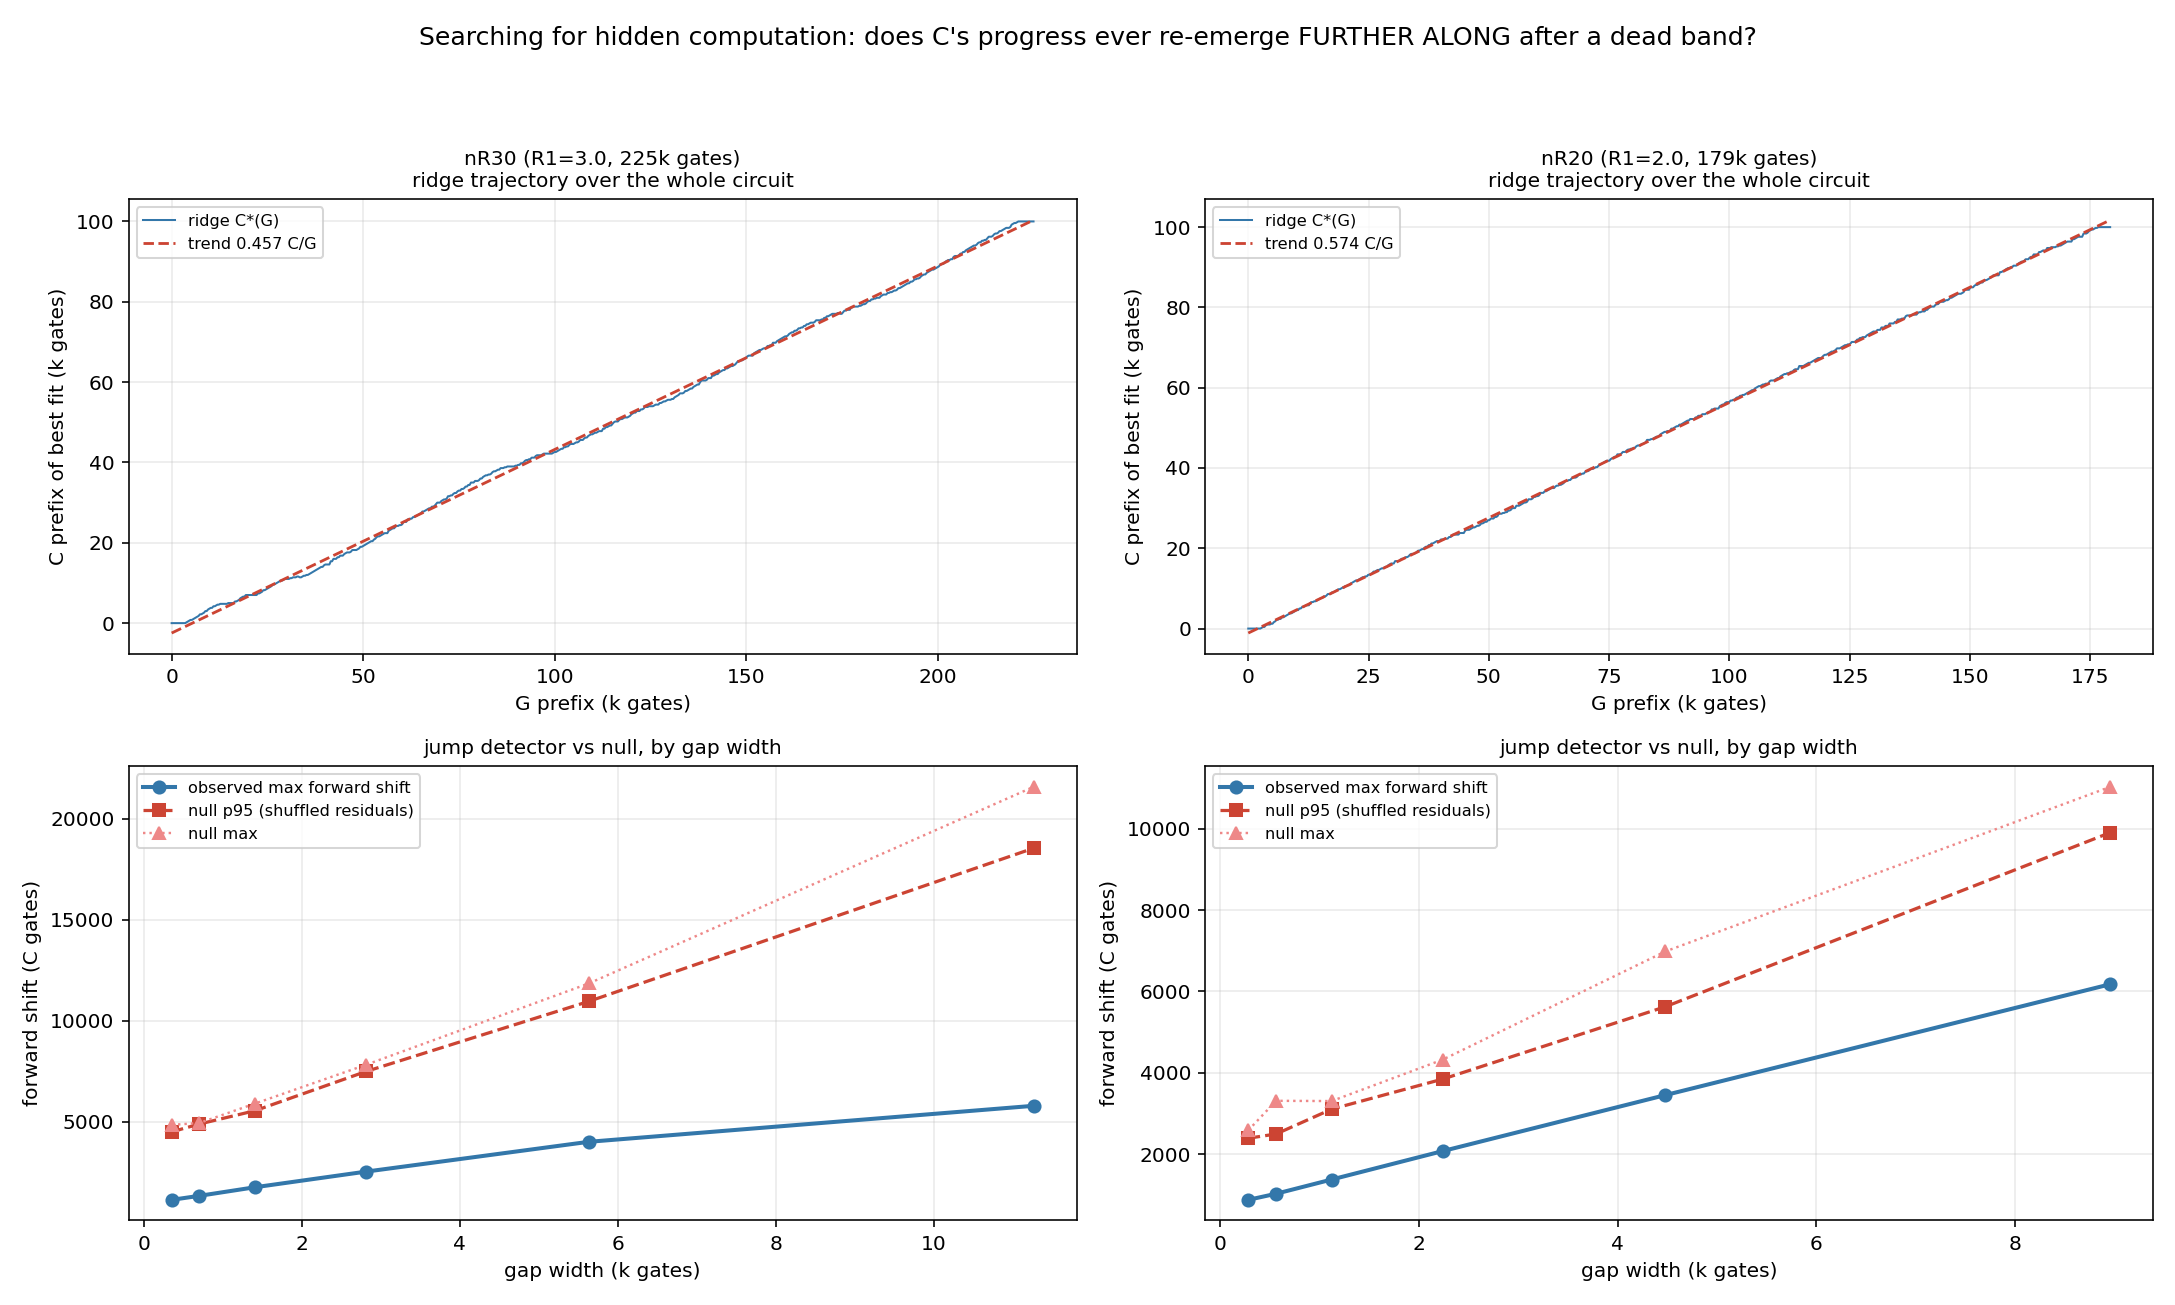
\includegraphics[width=\textwidth]{../reports/ancestry_20260728/jump_search_20260802.png}
\caption{Top: the ridge trajectory over the whole circuit against its fitted
trend. Bottom: observed maximum forward shift against the shuffled-residual
null, by gap width. The observed curve lies below the null everywhere.}
\end{figure}

\section{Incidental findings}

\begin{itemize}
\item \textbf{Ridge scatter scales with expansion.} \code{nR30}'s ridge
wobbles by 880 $C$-gates about its trend, \code{nR20}'s by 359. The more
expanded circuit localises its computational progress less tightly --- a
mild point in expansion's favour that the summary statistics miss.
\item \textbf{Mean $H$ rises with circuit size} (0.337 at 130k gates to
0.361 at 642k) while ridge \emph{depth} stays flat at 0.174--0.188. The
drift is dilution, not a weakening diagonal: per the standing directive,
read the plate by ridge, never by the mean.
\item \textbf{Two arms' strongest band sits in the first few percent} of
the circuit (R1=1.5, R1=2.5). Plausibly a head effect distinct from the
mid-circuit bands; not investigated.
\end{itemize}

\section{Tools added}

\begin{itemize}
\item \code{reports/hmap\_pixels.py} --- renders a plate at true 1:1, one
image pixel per matrix cell, with \code{--scale} for integer magnification,
\code{--gates A:B} to crop by $G$-gate index and \code{--annotate} to print
the numbers behind the pixels. Matplotlib's figure rendering resamples
plates and smears single-column features into their neighbours; this does
not.
\item \code{hmap\_affine --c-from/--c-to/--g-from/--g-to} --- restricts the
plate to a rectangle of prefix indices, so a dense \emph{local} plate costs
minutes instead of computing a dense global one.
\item \code{plot\_hmap\_ridge.py --no-ridge} --- draws the raw $H$ field
without the traced overlay, while still computing and printing the ridge
statistics.
\end{itemize}

\appendix
\clearpage
\section{The plates}

Every image below is rendered by \code{hmap\_pixels.py}: one image pixel per
matrix cell, integer replication only, no interpolation and no resampling.
Colour is fixed across the whole appendix --- $H = 0.10$ (red, leaking) to
$H = 0.45$ (blue, hidden) --- so panels are directly comparable. In every
plate rows are $C$ prefixes (top = start of the source computation) and
columns are $G$ prefixes (left = start of the mixed circuit).

\subsection{A resolution ladder on one circuit}

All five panels show the same object --- \code{nR30}, 225{,}014 gates
against a 100{,}000-gate source --- sampled at five resolutions. The point
of the ladder is that what a plate \emph{says} depends on how finely it is
cut: a coarse plate shows a clean diagonal and a handful of suspicious
columns; a fine one shows those columns are structured bands with
shoulders; a local one shows the diagonal itself has width and texture.

\begin{figure}[h]\centering
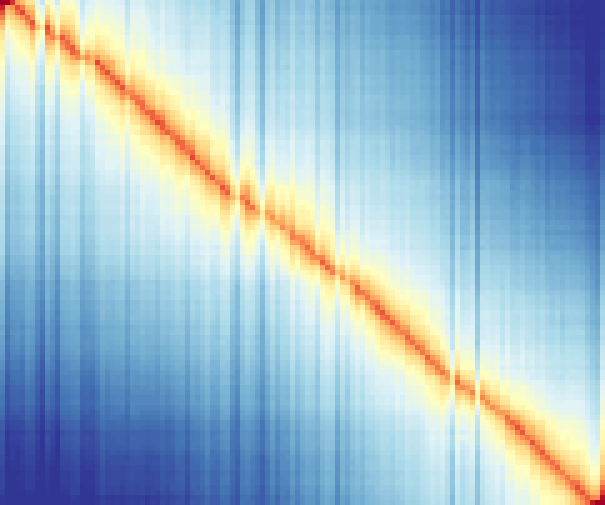
\includegraphics[width=0.72\textwidth]{../reports/ancestry_20260728/plates/lad1_coarse.png}
\caption{\textbf{Rung 1 --- global, coarse.} $101 \times 121$ cells;
$C$ step 1000, $G$ step 1876 gates. This is the plate the sweep was read
from. The diagonal is unmistakable; the pale columns are visible but
unresolved, each one cell wide.}
\end{figure}

\begin{figure}[h]\centering
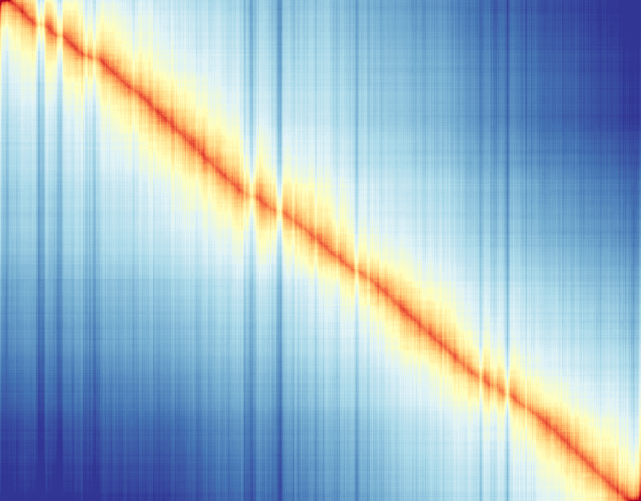
\includegraphics[width=0.9\textwidth]{../reports/ancestry_20260728/plates/lad2_tall.png}
\caption{\textbf{Rung 2 --- global, dense in $C$.} $501 \times 641$ cells;
$C$ step 200, $G$ step 352 gates, one pixel per cell at true 1:1. This is
the plate the hidden-computation search ran on: dense enough in $C$ that a
forward jump of a few hundred gates would be visible, over the whole
circuit rather than a window.}
\end{figure}

\begin{figure}[h]\centering
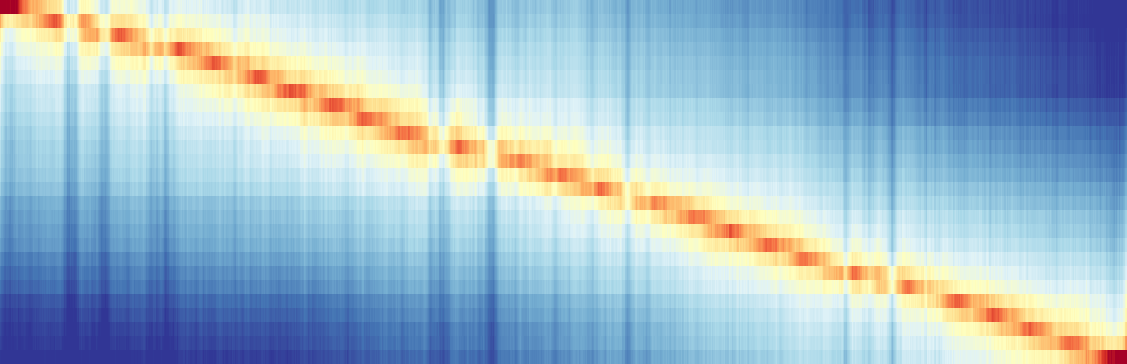
\includegraphics[width=\textwidth]{../reports/ancestry_20260728/plates/lad3_fine.png}
\caption{\textbf{Rung 3 --- fine in $G$, coarse in $C$.} $26 \times 1127$
cells; $G$ step 200 gates, $C$ step 4000, stretched $14\times$ vertically
(pixel replication, not interpolation). This is the cut that resolved the
band widths: the pale features are 200--2200 gates across with smooth
shoulders, not knife edges.}
\end{figure}

\begin{figure}[h]\centering
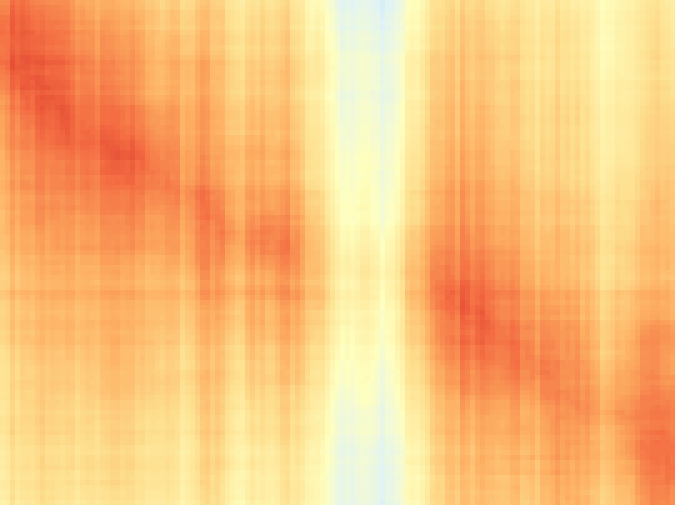
\includegraphics[width=0.8\textwidth]{../reports/ancestry_20260728/plates/lad4_band.png}
\caption{\textbf{Rung 4 --- local, dense in both.} $101 \times 135$ cells;
$C$ step 60, $G$ step 100 gates, over $C \in [39\text{k}, 45\text{k}]$,
$G \in [90.9\text{k}, 104.3\text{k}]$. At this scale the diagonal is a
textured structure of finite width rather than a line.}
\end{figure}

\begin{figure}[h]\centering
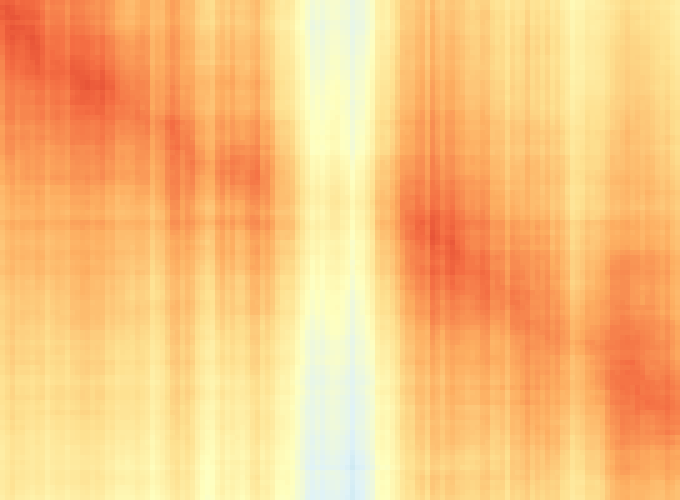
\includegraphics[width=0.8\textwidth]{../reports/ancestry_20260728/plates/lad5_z2B.png}
\caption{\textbf{Rung 5 --- local, aspect-matched.} $100 \times 136$ cells
over $C$ 6000 gates $\times$ $G$ 13{,}500 gates, i.e.\ a window whose sides
are in the circuit's own $2.25$ size ratio, so the ridge runs corner to
corner instead of sweeping out of frame. Compare with rung 4: the same
material, framed correctly.}
\end{figure}

\clearpage
\subsection{One band from each profile arm}

Each panel is that arm's own strongest band, in a window aspect-matched to
that arm's own size ratio, at $C$ step 60 gates. Same colour scale
throughout ($0.10$--$0.35$ here, since these local windows never reach the
global extremes). The bands look alike across very different runs --- the
$6.4\times$-expanded twist-heavy circuit included --- which is the visual
counterpart of the finding that no profile parameter changes the plate.

\begin{figure}[h]\centering
\begin{tabular}{cc}
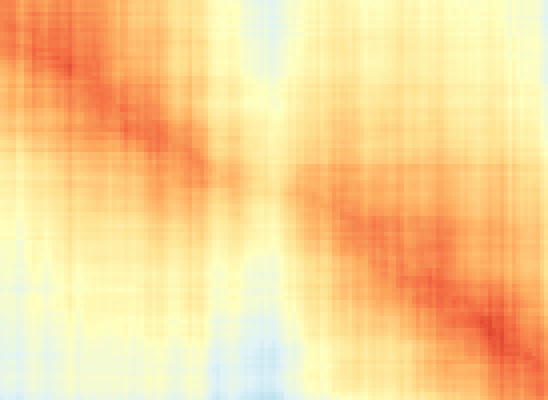
\includegraphics[width=0.44\textwidth]{../reports/ancestry_20260728/plates/app_band_notwist.png} &
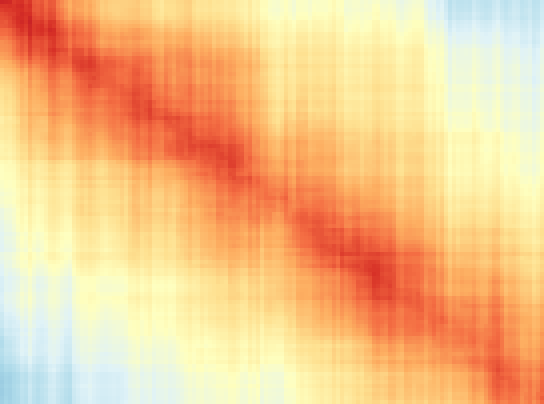
\includegraphics[width=0.44\textwidth]{../reports/ancestry_20260728/plates/app_band_nR15.png} \\
{\small no twist (130k gates, ratio 1.30)} & {\small R1=1.5 (149k, 1.49)} \\[4pt]
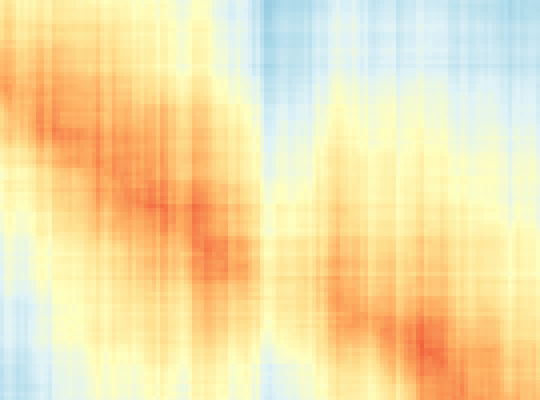
\includegraphics[width=0.44\textwidth]{../reports/ancestry_20260728/plates/app_band_nR20.png} &
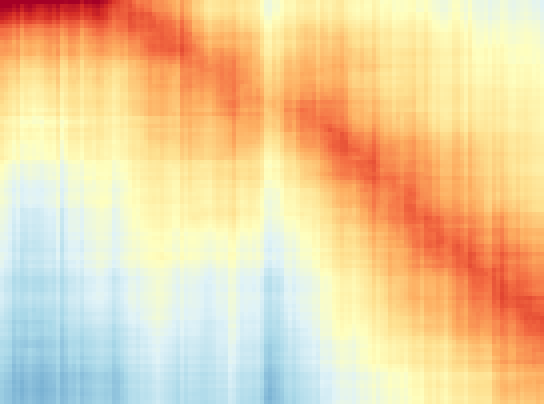
\includegraphics[width=0.44\textwidth]{../reports/ancestry_20260728/plates/app_band_nR25.png} \\
{\small R1=2.0 (179k, 1.79)} & {\small R1=2.5 (199k, 1.99)} \\
\end{tabular}
\end{figure}

\begin{figure}[h]\centering
\begin{tabular}{cc}
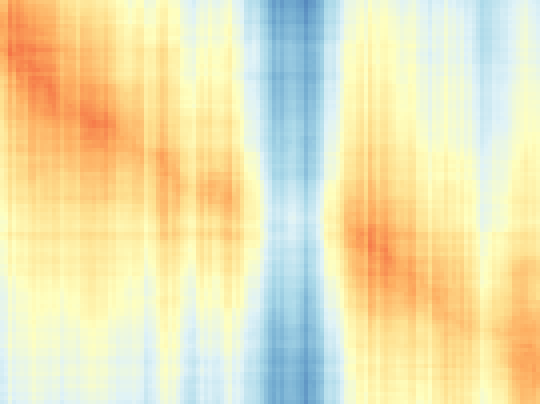
\includegraphics[width=0.44\textwidth]{../reports/ancestry_20260728/plates/app_band_nR30.png} &
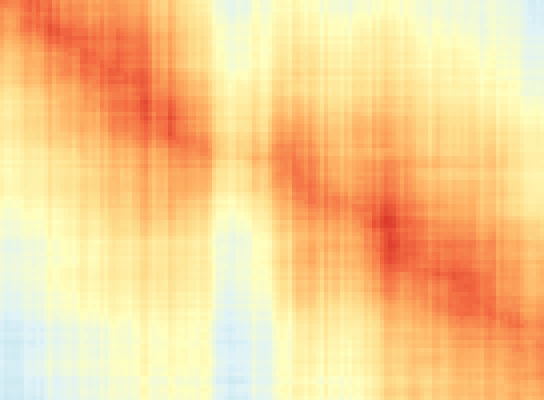
\includegraphics[width=0.44\textwidth]{../reports/ancestry_20260728/plates/app_band_nR20_fast.png} \\
{\small R1=3.0 (225k, 2.25)} & {\small short hold (162k, 1.62)} \\[4pt]
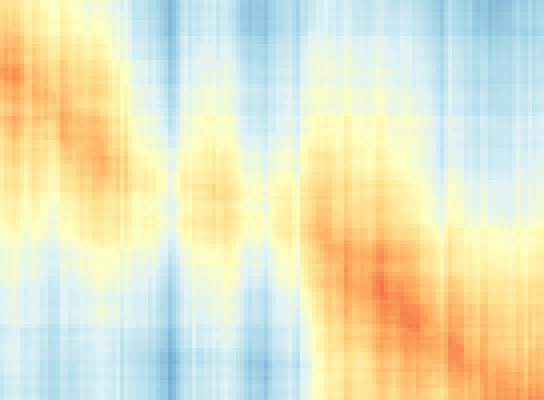
\includegraphics[width=0.44\textwidth]{../reports/ancestry_20260728/plates/app_band_nR20_slow.png} &
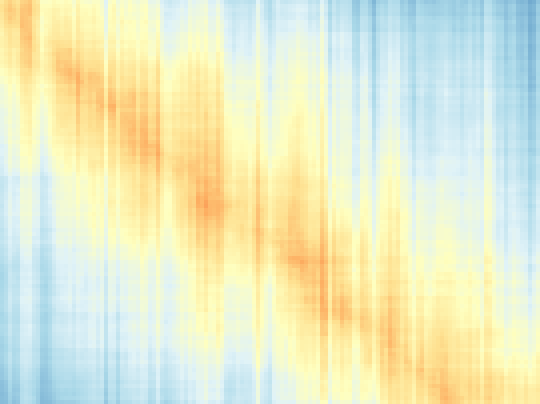
\includegraphics[width=0.44\textwidth]{../reports/ancestry_20260728/plates/app_band_nR20_tw5.png} \\
{\small long hold (198k, 1.98)} & {\small 10$\times$ twist (642k, 6.42)} \\
\end{tabular}
\end{figure}

\end{document}
